\section{Reader's guide to the page and the repository}\label{sec:guide}

The graph lives at \live{} (source and data at \repo). This section explains the page from the screen inward, for a reader who has not seen a GEN page before. Figure~\ref{fig:ui} is the page at Step~6 with the controls numbered.

\begin{figure}[htbp]\centering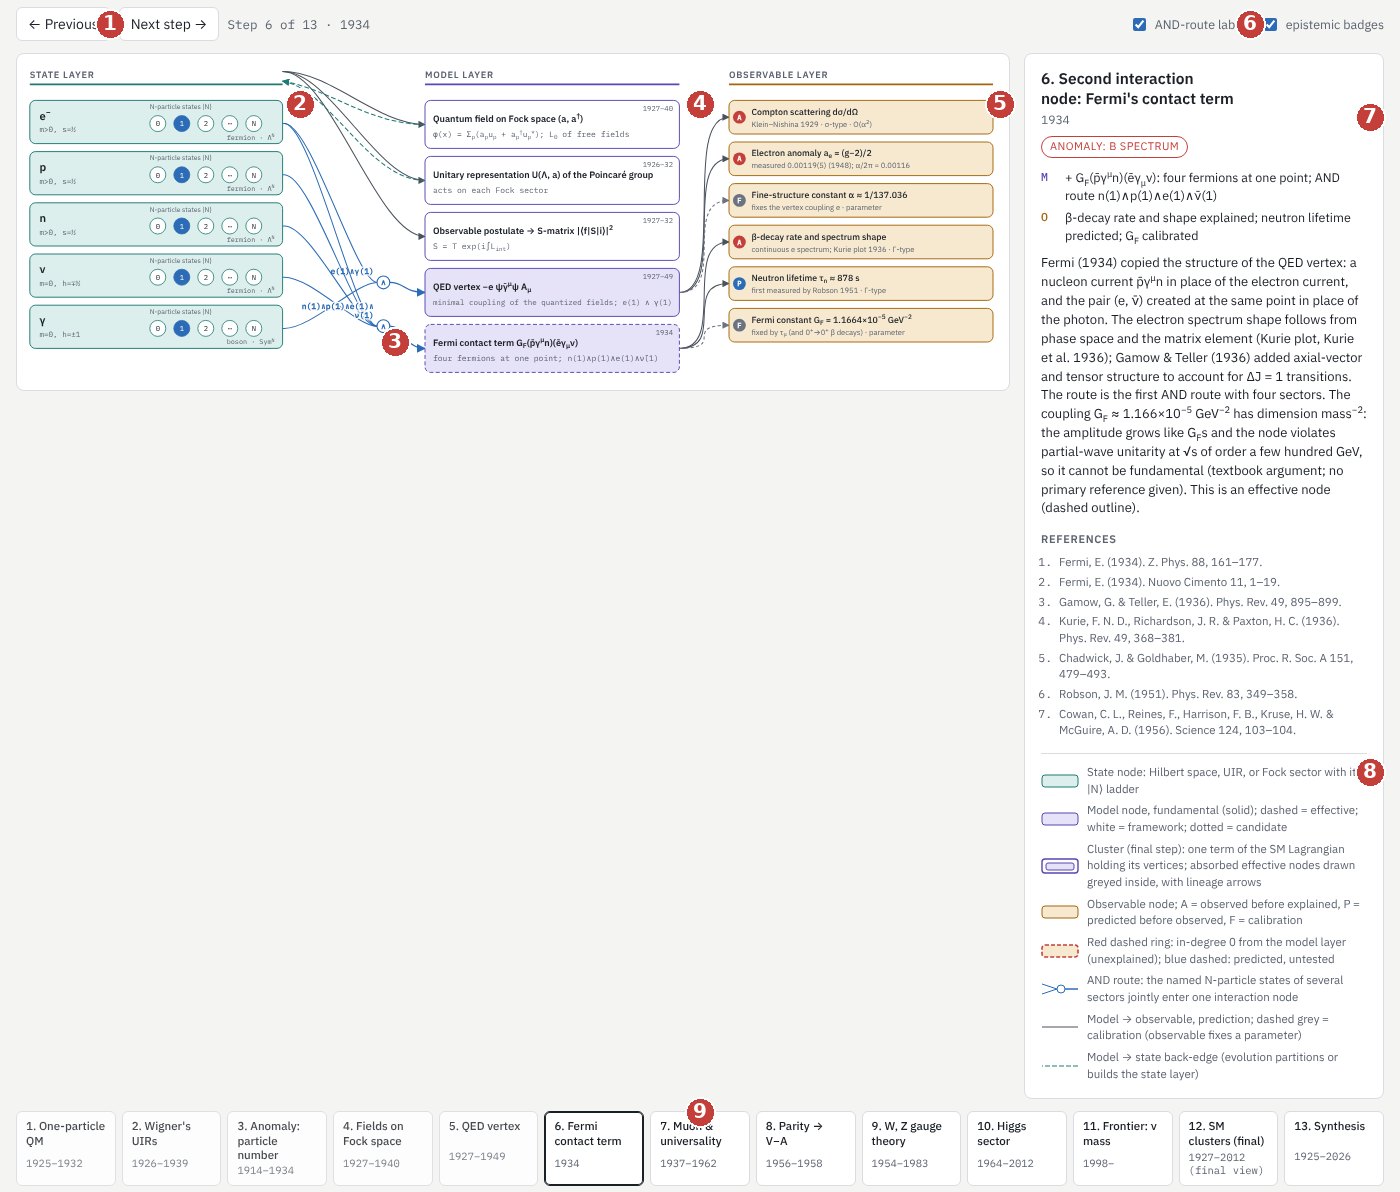
\includegraphics[width=\linewidth]{ui_annotated.png}
\caption{The page at Step 6, with its parts numbered: (1) step controls, (2) state column, (3) an AND junction, (4) model column, (5) observable column, (6) display toggles, (7) the rail with the step text and references, (8) the legend, (9) the step timeline.}\label{fig:ui}\end{figure}

\subsection{Reading one step}
\begin{enumerate}
\item \textbf{Step controls (1).} ``Next step'' and ``Previous'' move through the \nSteps{} steps; the left and right arrow keys do the same. The counter shows the step number and its years. Each step has its own address (\texttt{\#step-7}), so a step can be bookmarked or sent.
\item \textbf{State column (2).} From Step~4 on, each box is one field sector: its name, its Wigner label ($m>0$, $s=\tfrac12$, \dots), its statistics (fermion $\Lambda^N$ or boson Sym$^N$), and its occupation ladder $0,1,2,\dots,N$. A blue filled rung is an occupation number that enters a route in the current step. In Steps~1--3 the column holds the Hilbert space and the representation classes instead.
\item \textbf{AND junction (3).} Blue lines leave the rungs of several sectors and meet at a circle marked $\wedge$; one blue arrow continues into a model node. The label beside the junction names the legs, e.g.\ $n(1)\wedge p(1)\wedge e(1)\wedge\bar\nu(1)$. The toggle ``AND-route labels'' (6) hides these labels when the picture is dense.
\item \textbf{Model column (4).} Framework nodes are white; interaction nodes are violet, dashed if effective, dotted if candidate. Each node shows its years, its name and its formula. In Step~12 the nodes are grouped into clusters, one per Lagrangian term, with the absorbed effective nodes greyed inside.
\item \textbf{Observable column (5).} Each chip carries a badge (A, P or F, see the legend) and a one-line value or reference. A red dashed ring means the observable has no model edge in this step; a blue dashed ring means a prediction not yet tested.
\item \textbf{Rail (7).} The rail shows the step: title, years, the driver of the step (anomaly, symmetry, model response, prediction, clustering), what changed in each layer, the narrative, and the numbered references. \textbf{Clicking a node} replaces the rail with that node's page: formula, description, instances, its edges in this step with their relations, and its references. \textbf{Hovering an edge} highlights it and shows its mathematical relation in a tooltip; \textbf{clicking an edge} opens the relation in the rail. ``Back to step'' or the Escape key returns to the step text.
\item \textbf{Legend (8)} and \textbf{timeline (9).} The legend is repeated under every step text. The timeline at the bottom lists all steps with their years and jumps to any of them.
\item \textbf{Step 13, the method in action.} The last step replaces the graph with the synthesis: the method cycle on the left, the compact schematic on the right, and the operation log below (Figures~\ref{fig:m4}--\ref{fig:m12}). Use the numbered buttons or the arrows to choose a step, or press Play to run all twelve; hover a node in the schematic for its name, hover a phase in the cycle for its definition. Below it are the count charts and the table of changes per layer.
\end{enumerate}

\subsection{How to study the history with the page}
A productive order for a student is: read Step~1 and Step~2 for the kinematics; at Step~3 look for the red ring and ask what kind of model node could reach it before pressing ``Next''; at Step~4 click the field node and the sector boxes to see the back-edge and the ladders; from Step~5 on, for every new violet node, hover its route and its observable edges and read the relation on each edge (this is where the physics is); at Steps~8 and~9 watch the model column shrink and grow; at Step~12 open the gauge--fermion cluster and follow the lineage edges from Fermi's node to the charged current; finally read Step~13 for the counts.

\subsection{Versions}
The repository keeps every version. \texttt{v1.0/} is the first release (eleven graph steps and a synthesis), \texttt{v1.1/} adds the clustered final step, \texttt{v1.2/} adds the method-in-action synthesis view, and \texttt{latest/} always opens the newest version. Each page has a version bar at the top that links to the other versions; earlier versions show a notice pointing to the newest. The landing page lists what changed in each version.

\subsection{Data and derived files}
\begin{itemize}
\item \texttt{data/v1.2\_sm\_epistemic\_graph.json}: the full graph (nodes, references, steps with edges, routes, groups, clusters, and the phases and operations of each step), described in Appendix~\ref{app:data}. The page reads the same data embedded in its HTML.
\item \texttt{data/statistics.json}: per-step counts (nodes per layer, routes, unexplained observables).
\item \texttt{catalog.md}: every node, edge and route of every step as Markdown tables, with the references.
\item \texttt{tools/build\_derived.py}: regenerates the statistics, the catalogue, and every table and number of this paper from the JSON, so that the paper cannot drift from the graph.
\item \texttt{paper/}: this document, compiled with XeLaTeX (\texttt{latexmk -xelatex main.tex}).
\end{itemize}

\subsection{How to extend the graph}
A new node is a new entry in the \texttt{NODES} dictionary of the page (or of the JSON) with its layer, kind, label, years, description and references. A new step is a new entry in \texttt{STEPS} that lists the node identifiers of each layer, the edges with their relations, the routes with their legs, and, if the step removes nodes, the \texttt{morph} map that says which node each removed one animates into. To add the strong sector, for example, one would add the sectors $n$, $p$ (already present) and $\pi$, the Yukawa pion--nucleon node with the route $n(1)\wedge p(1)\wedge\pi(1)$, its observables (nucleon--nucleon and pion--nucleon cross sections, the deuteron), and later the quark and gluon sectors with the QCD vertex and the lineage edge that absorbs the pion node as a low-energy effective theory. After editing, \texttt{python3 tools/build\_derived.py} rebuilds the derived files, and a new version folder keeps the previous page intact. The GEN rule for edges applies: a relation the literature establishes must be an edge, so two nodes stay unconnected only when no edge can be made from the literature, and a missing edge is either a defect to report or a research target.
